In 1877, and extended in 1926 by Volmer and Weber, Gibbs originally developed classical nucleation theory (CNT) for liquid formation in supercooled vapor \cite{debenedetti1996metastable}.  The theory was later extended to crystal formation in supercooled liquids \cite{debenedetti1996metastable}.  Gibbs theorized that, in order for a new phase to form in a bulk phase, a free energy barrier must be overcome for the creation of a nucleus site of the new phase.  Classical nucleation theory was the first framework to argue that the kinetic rates involved in nucleation depended on the exponential of a free energy activation barrier \cite{debenedetti1996metastable}.  This idea is pictorially displayed in Figure \ref{CNT} for the formation of a crystal in a bulk liquid.  

\begin{figure}[h]
	\centering
%	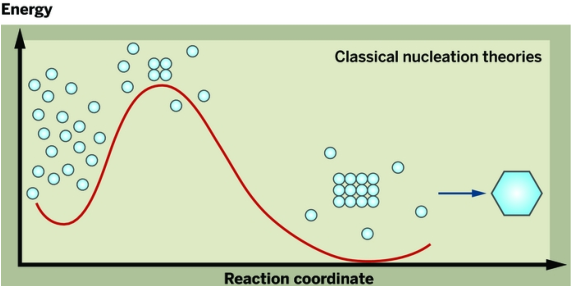
\includegraphics[width = .7\textwidth]{./Figures/cnt.pdf}
	\includegraphics[width = .5\textwidth]{./Figures/CNT/nucleation.png}
	\caption[Figure to show a schematic drawing of classical nucleation theory.  The figure shows the prevalent idea behind classical nucleation: nucleation is dominated by a single free-energy barrier that requires an activated event to overcome.  The figure shows to the left of the barrier the system is in the liquid phase, at the top of the barrier a critical nucleus site is formed of the crystal phase, and to the right is the fully developed crystal phase.  Generally, if a nucleation site as large as the critical size is created, the crystal phase will become ubiquitous in the system, but if the nucleation site is smaller, the liquid phase will remain ubiquitous.]{Figure to show a schematic drawing of classical nucleation theory.  The figure shows the prevalent idea behind classical nucleation: nucleation is dominated by a single free-energy barrier that requires an activated event to overcome.  The figure shows to the left of the barrier the system is in the liquid phase, at the top of the barrier a critical nucleus site is formed of the crystal phase, and to the right is the fully developed crystal phase.  Generally, if a nucleation site as large as the critical size is created, the crystal phase will become ubiquitous in the system, but if the nucleation site is smaller, the liquid phase will remain ubiquitous. \cite{debenedetti1996metastable}}
	\label{CNT}
\end{figure}

Figure \ref{CNT} shows a schematic drawing of the CNT framework \cite{debenedetti1996metastable}.  The figure shows that a system begins in a high energy amorphous state, and is separated from the stable crystal state by a large energy barrier \cite{debenedetti1996metastable}.  This barrier represents the energy cost for the system to enter a two phase state \cite{debenedetti1996metastable}.  CNT argues that a system in the absence of surfaces and impurities will under go random density fluctuations, resulting in sites of the more stable phase \cite{debenedetti1996metastable}.  If the new phase site is sufficiently large, the system will without bounds transition to the new phase.  However, if the site is not sufficiently large, the site will collapse back to the original phase.  CNT argues that nucleation is an activated process.  In this chapter, we will show how CNT approximates the height of this energy barrier and utilizes the barrier to estimate the nucleation rate.  Next, we will present some promising results employing CNT.  Lastly, discussion of the short comings of the framework, and how the theory can be improved will be presented.

\section{Estimating the Energy Barrier}
In the original theory, a liquid phase nucleation site develops in a bulk supercooled vapor \cite{mutaftschiev2001atomistic}.  In this theory, the nucleus is assumed to be spherical in shape and to be much larger than the atomic dimensions of the material (the radius of the nucleus is assumed larger than a few molecular diameters).  As a result of a new phase, an interface develops between the two phases, a liquid-vapor phase in the original theory.  Because of the aforementioned assumptions, this interface is treated macroscopically, despite being a microscopic feature.  Therefore, when a nucleation site forms, there is a free-energy penalty for the formation of the nucleation site, due to the introduction of this interface.  By assuming the interface can be treated macroscopically, the interface free energy is calculated by the surface tension of the new phase \cite{mutaftschiev2001atomistic}.
\begin{equation}
	\Delta G_{i} = A\gamma 
\end{equation}
where $A$ is the area of the nucleation site, and $\gamma$ is the surface tension of the liquid.

On the other hand, there is also a free energy difference from the creation of a new phase.  The free energy of the formation of a new phase is calculated from the chemical potential of the two phases \cite{mutaftschiev2001atomistic}.  Each phase has a chemical potential, $\mu$.
\begin{equation}
	\Delta G_{f} = V\rho\Delta \mu
\end{equation}
where $V$ is the volume of the nucleation site, $\rho$ is the atomic density, and $\Delta \mu$ is the difference in the chemical potential defined as
\begin{equation}
	\Delta \mu = \mu_{new} - \mu_{old}
\end{equation}
where $new$ and $old$ indicate the nucleation phase and the bulk phase, respectively.

Because the nucleation site is assumed spherical the area and the volume of the nucleation site is known as
\begin{equation}
	\begin{split}
		A &= 4\pi r^2\\
		V &= \frac{4}{3}\pi r^3 
	\end{split}
\end{equation}
where $r$ is the radius of the nucleation site \cite{mutaftschiev2001atomistic}.  Thus, the free energy barrier of nucleation as a function of nucleation site radius is determined by the following equation
\begin{equation}
	\Delta G(r) = \Delta G_{f}(r) + \Delta G_{i}(r) = \frac{4}{3}\pi r^3\rho \Delta \mu + 4\pi r^2\gamma
\end{equation}
This is pictorially displayed in Figure \ref{cnt_energy}.

\begin{figure}[h]
	\centering
	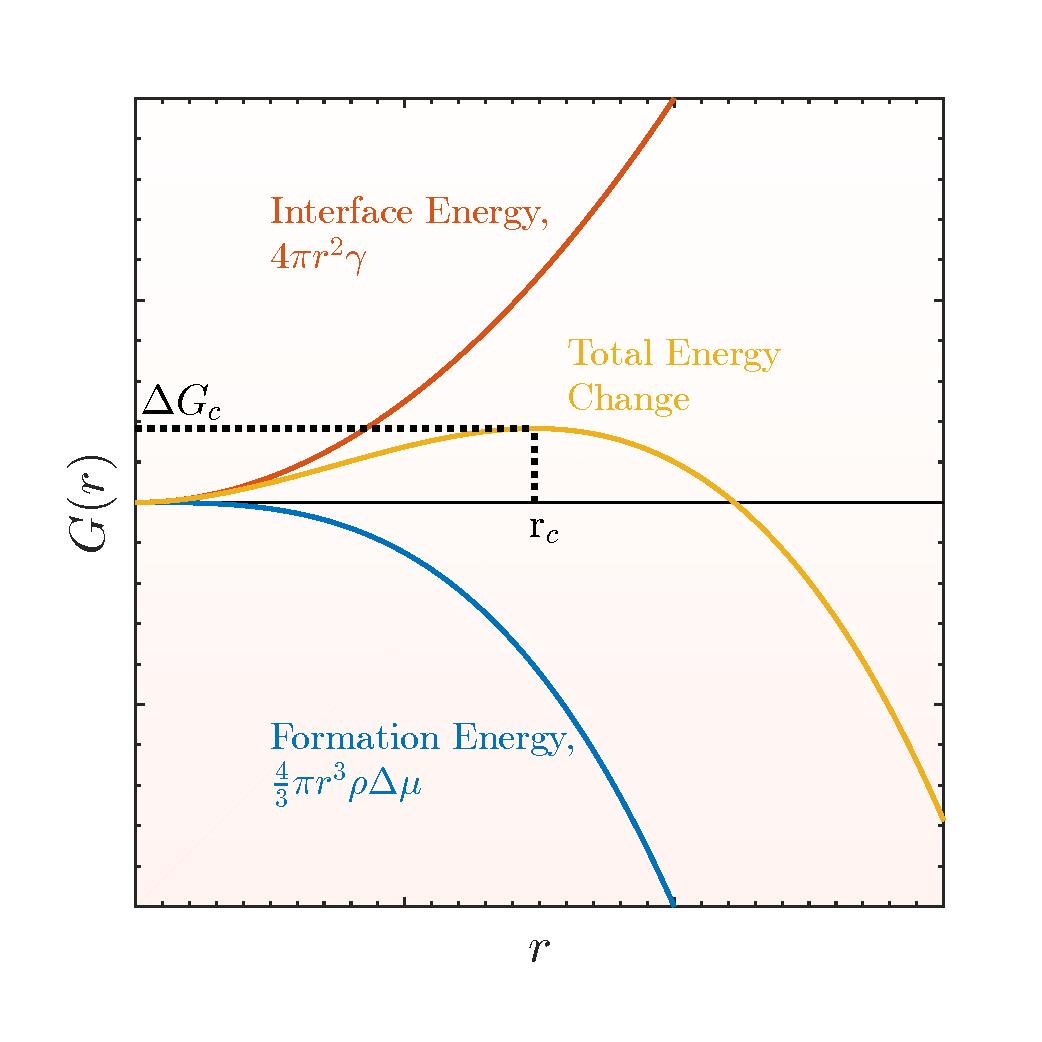
\includegraphics[width = .5\textwidth]{./Figures/CNT/cnt_energy.pdf}
	\caption[Gibbs free energy plotted as a function of nucleation cluster radius.  The blue line shows the energy change due to the formation of a nucleation site.  The orange line shows the energy change introduced by the interface between the two phases of the bulk phase and the nucleation site phase.  The yellow line shows the total of the formation energy and the interface energy.  The figure shows there is a critical value (maximum value) for the total of the two.  If the nucleation site has a radius less than the critical size, then the nucleation site will dissipate to reduce the Gibbs free energy of the system.  Comparatively, if the site is greater than the critical radius, then the nucleation site will preferentially grow to reduce the Gibbs free energy.]{Gibbs free energy plotted as a function of nucleation cluster radius.  The blue line shows the energy change due to the formation of a nucleation site.  The orange line shows the energy change introduced by the interface between the two phases of the bulk phase and the nucleation site phase.  The yellow line shows the total of the formation energy and the interface energy.  The figure shows there is a critical value (maximum value) for the total of the two.  If the nucleation site has a radius less than the critical size, then the nucleation site will dissipate to reduce the Gibbs free energy of the system.  Comparatively, if the site is greater than the critical radius, then the nucleation site will preferentially grow to reduce the Gibbs free energy. \cite{debenedetti1996metastable}}
	\label{cnt_energy}
\end{figure}

Figure \ref{cnt_energy} shows the free energy for the interface between the two phases, the formation of a new phase, and the total free energy change \cite{debenedetti1996metastable}.  In classical nucleation theory, while in equilibrium, a bulk material will undergo thermal and density fluctuations, which will lead to nucleation sites of the new phase \cite{mutaftschiev2001atomistic}.  These nucleation sites are assumed to have a certain radius.  If the radius is smaller than the critical radius, $r_{c}$, the site has not overcome the free energy barrier and the surface tension term will dominate causing the nucleation site to reduce back to the original phase \cite{mutaftschiev2001atomistic}.  Alternatively, if the nucleation site radius is equal to $r_{c}$ or larger than the site has overcome the free energy barrier and the formation energy will dominate \cite{mutaftschiev2001atomistic}.  As a result, since the new phase is energetically preferential at this temperature, the new phase will grow throughout the system \cite{debenedetti1996metastable}.  

The critical radius can simply be calculated by determining the derivative of the free energy of nucleation and setting the derivative to zero.
\begin{equation}
	\frac{d \Delta G(r)}{d r}\Bigg{|}_{r=r_{c}} = 4\pi\rho\Delta\mu r_{c}^2 + 8\pi \gamma r_{c} = 0
\end{equation}
Solving this for $r_{c}$, results in
\begin{equation}
	r_{c} = -\frac{2\gamma}{\rho\Delta\mu} = -\frac{2\gamma v}{\Delta\mu}
\end{equation}
where $v$ is the atomic specific volume \cite{Vehkamaki2006}.  The critical radius is negative here because $\Delta\mu$ is negative if the new phase is energetically favorable \cite{Vehkamaki2006}.  Thus,
\begin{equation}
\begin{split}
r_{c} = \frac{2\gamma v_l}{|\Delta\mu|} \quad \mu_{new} < \mu_{old} \\
r_{c} = -\frac{2\gamma v_l}{|\Delta\mu|} \quad \mu_{old} < \mu_{new} \\
\end{split}
\end{equation}
Thus, if the new phase is not energetically favorable, the critical radius is negative and, as a result, the new phase will never emerge \cite{Vehkamaki2006}.  

\begin{figure}[h]
	\centering
	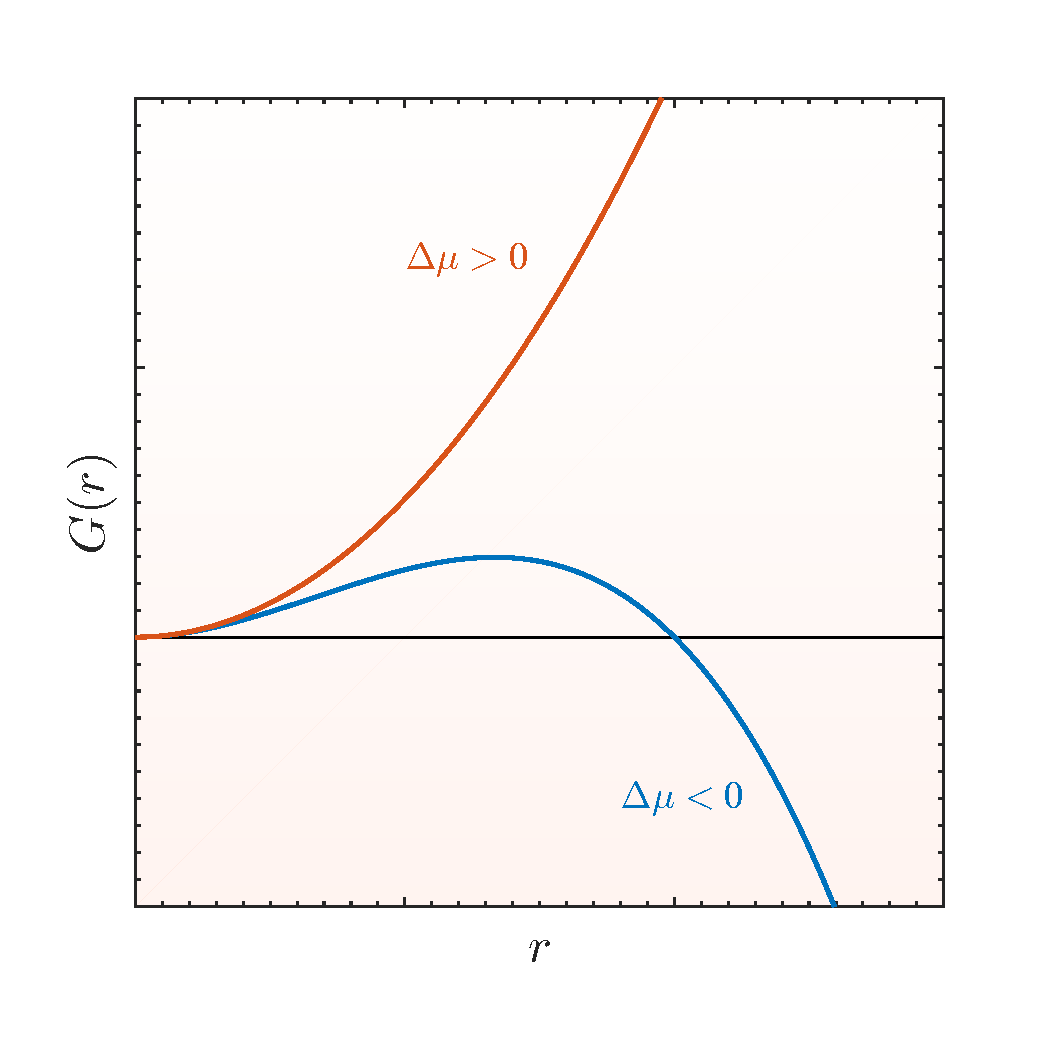
\includegraphics[width = .5\textwidth]{./Figures/CNT/cnt_mu.pdf}
	\caption[Gibbs free energy plotted as a function of nucleation cluster radius.  The blue line is identical to the yellow line in Figure \ref{cnt_energy}.  When the difference in the chemical potential is negative (new phase is more stable), the Gibbs free energy takes the shape of the blue line.  However, if the difference in the chemical potential is positive (new phase is less stable), the Gibbs free energy takes the shape of the orange line, and the formation of the new phase is highly improbable.  If the difference in the chemical potential is zero, the two phases are in equilibrium, and neither phase will preferentially grow.]{Gibbs free energy plotted as a function of nucleation cluster radius.  The blue line is identical to the yellow line in Figure \ref{cnt_energy}.  When the difference in the chemical potential is negative (new phase is more stable), the Gibbs free energy takes the shape of the blue line.  However, if the difference in the chemical potential is positive (new phase is less stable), the Gibbs free energy takes the shape of the orange line, and the formation of the new phase is highly improbable.  If the difference in the chemical potential is zero, the two phases are in equilibrium, and neither phase will preferentially grow \cite{Vehkamaki2006}. }
	\label{cnt_mu}
\end{figure}

The chemical potential dependence is also pictorially displayed in Figure \ref{cnt_mu} \cite{Vehkamaki2006}.  This figure shows the total free energy for a nucleation site as function of nucleation site radius \cite{Vehkamaki2006}.  The figure shows that if the new phase is energetically favorable, $\mu_{new} < \mu_{old} $, there is an energy barrier that must be over come.  However, if the opposite is true, $\mu_{new} > \mu_{old}$, then the free energy increases to infinity as the radius goes to infinity, and as a result, the new phase will never develop in the system.  Lastly, if the new phase is assumed to be energetically favorable and the critical radius is positive, the free energy barrier can be computed as
\begin{equation}\label{G_critical}
\Delta G_{c} (r_{c}) = -\frac{4}{3}\pi \frac{8\gamma^3 v_l^3}{\Delta\mu^3}\frac{\Delta\mu}{v_l} + 4\pi\frac{4\gamma^2v_l^2}{\Delta\mu^2}\gamma = \frac{16\pi}{3}\frac{\gamma^3 v_l^2}{\Delta \mu^2}
\end{equation}
Equation \ref{G_critical} is the critical radius when the nucleation phase is energetically favorable \cite{debenedetti1996metastable}.  If the bulk phase is energetically favorable, then the free-energy barrier is infinite for positive values of the nucleation radius.  Both the critical radius and free energy barrier are displayed on Figure \ref{cnt_energy} \cite{debenedetti1996metastable}.  Thus, the free energy barrier is a function of the surface tension, the atomic specific volume, and the difference in chemical potential, which are all macroscopic equilibrium variables.  The goal of most nucleation studies is to predict this free energy barrier in order to calculate the nucleation rate with CNT \cite{debenedetti1996metastable}\cite{Oxtoby1992}.  The nucleation rate is then calculated from the free energy barrier with the following equation
\begin{equation}
J(T) = N_sZf\exp\left(\frac{-\Delta G_c}{k_BT}\right)
\end{equation}
where $J$ is the nucleation rate, $N_s$ is the number of nucleation sites formed per unit volume, $Z$ is the Zeldovich factor, and $f$ is the attachment rate \cite{Vehkamaki2006}\cite{Espinosa2016}.  The Zeldovich factor determines the fraction of nucleation sites that reach the critical size that continue to grow in size rather than dissolve back to the bulk phase \cite{Vehkamaki2006}.  The Zeldovich factor is determined by thermal fluctuations \cite{Vehkamaki2006}.  A nucleation site of critical size can either fluctuate to grow beyond the critical size, or fluctuate to lose atoms resulting in the nucleation site returning to the bulk phase.  The attachment rate, $f$, is the rate of atoms that contact the nucleation site that add to the nucleation site \cite{Auer2001}.  Many recent works use the approximation of Auer and Frenkel to estimate the attachment rate
\begin{equation}
	f = \frac{\langle (N(t) - N_c)^2\rangle}{2t}
\end{equation}
where $N(t)$ is the number of atoms in the nucleation site, $N_c$ is the number of atoms in a critical nucleation site, and $t$ is time \cite{Auer2001}\cite{Espinosa2016}.  This provides an estimate to the attachment rate.  Thus, most simulations of nucleation make approximations to estimate the free energy barrier, the Zeldovich factor, and the attachment rate.  $N_s$ is determined as the specific volume since in a simulation only one nucleation event will occur in a simulation cell.

\section{Inaccuracies of CNT Application}
The difficulty of estimating the nucleation free-energy barrier with CNT is that a method to compute the nucleation site size is required.  Traditionally, many would turn to MD or MC simulations to determine the nucleation site size, however, MD simulations are limited by temporal restraints that prevent a nucleation event from occurring within the timescale of an MD simulation.  MD simulations are typically on the scale of a few thousand atoms and at most the microsecond time scale.  With these numbers the probability of simulating a nucleation event from equilibrium is near impossible.  As a result, one highly successful method to estimate the nucleation site size is to begin an MD simulation with a nucleation site of size N \cite{Espinosa2016}\cite{Sanz2013}.  Then, by performing MD, the nucleation site will either grow or shrink, and with this, the critical radius can be estimated \cite{Espinosa2016}\cite{Sanz2013}.  However, the issue with this method is it requires thousands of simulations to approximate the free-energy barrier for one temperature \cite{Espinosa2016}.  Despite this computational intensity, the method showed promise when applied to both liquid and crystal nucleation \cite{Espinosa2016}.

Classical nucleation theory was first applied to the nucleation of a liquid phase in a vapor phase, and showed promising results.  For this phase transition, CNT made highly accurate predictions.  CNT used in tandem with MD and MC simulations were able to accurately predict the nucleation rate of supercooled vapors.  However, when extended to crystal nucleation in a liquid phase, the short comings of CNT soon became evident.  Figure \ref{cnt_failure} shows comparison plots between CNT and experimental values \cite{Vehkamaki2006}. 

\begin{figure}[h]
	\centering
	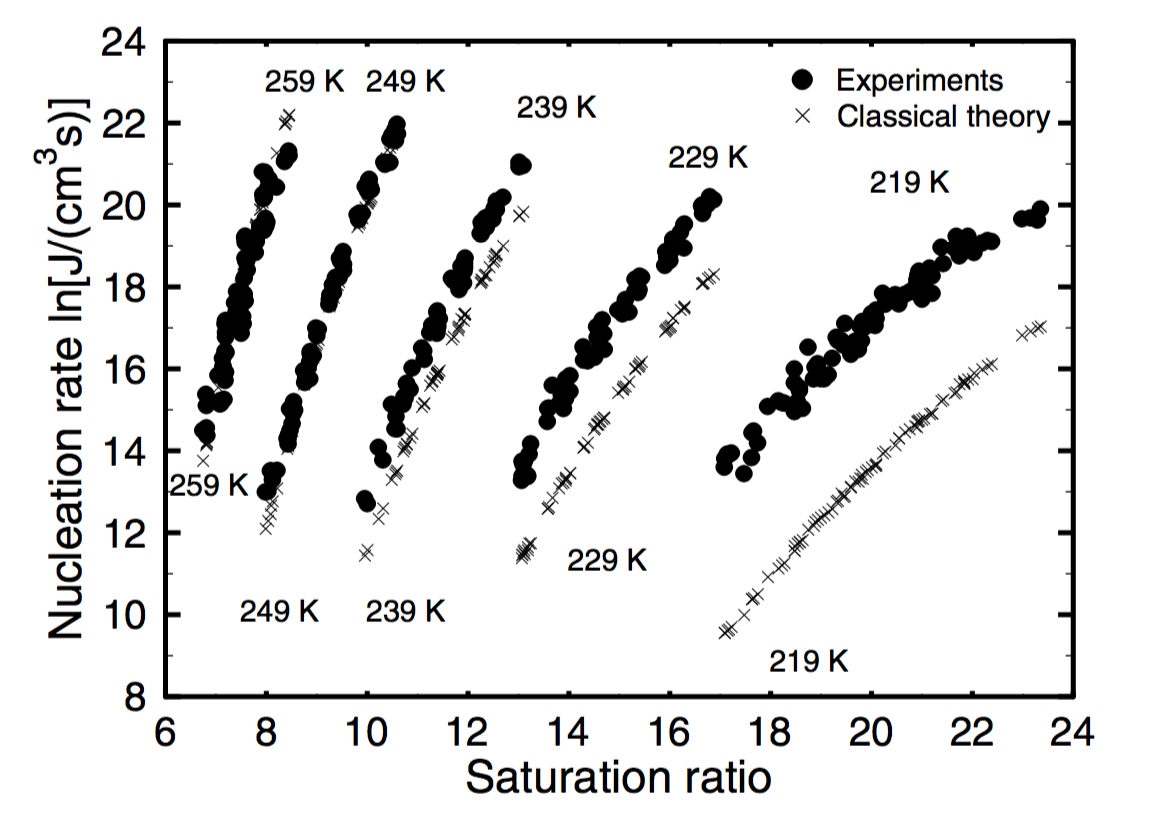
\includegraphics[width = .45\textwidth]{./Figures/CNT/cnt_failure.png}
	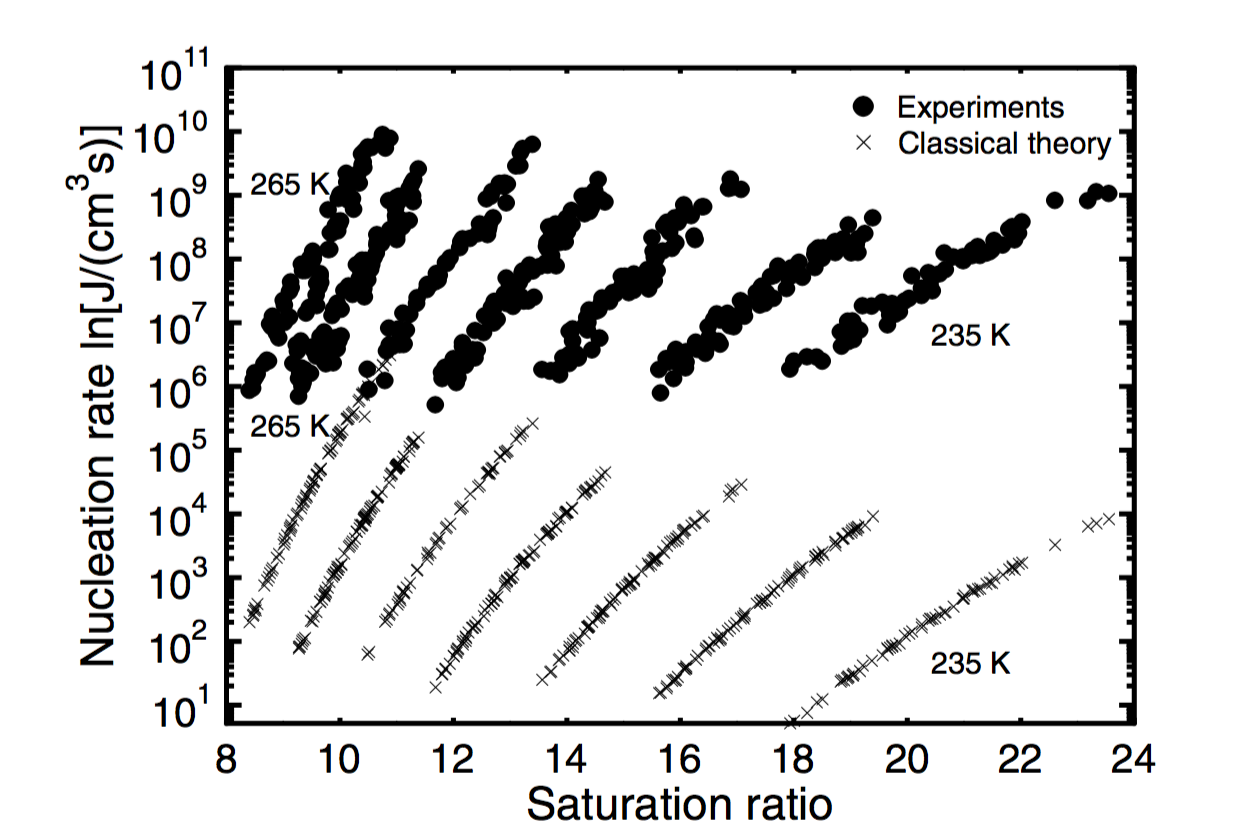
\includegraphics[width = .49\textwidth]{./Figures/CNT/cnt_failure_2.png}
	\caption[Figures showing the comparison of experiential results with classical nucleation results.  The figures show the nucleation rate plotted versus saturation ratio for several temperatures.  The left figure are results for water and the right figure are results for 1-pentanol.  The two figures show that classical nucleation theory accurately captures the shapes of the curves as a function of saturation ratio for fixed temperatures.  However, the exact estimation by CNT is orders of magnitude from the experimental values for lower temperatures in water and all temperatures in 1-pentanol.]{Figures showing the comparison of experiential results with classical nucleation results.  The figures show the nucleation rate plotted versus saturation ratio for several temperatures.  The left figure are results for water and the right figure are results for 1-pentanol.  The two figures show that classical nucleation theory accurately captures the shapes of the curves as a function of saturation ratio for fixed temperatures.  However, the exact estimation by CNT is orders of magnitude from the experimental values for lower temperatures in water and all temperatures in 1-pentanol \cite{Vehkamaki2006}.}
	\label{cnt_failure}
\end{figure}

Figure \ref{cnt_failure} shows the CNT prediction for water and 1-pentanol \cite{Vehkamaki2006}.  This figure shows that the relationship between nucleation rate and saturation ratio agree well between experiments and CNT.  However, the two methods agree well for water at 259 K, but as the temperature is decreased, the agreement soon fades.  Similarly, for a more complex system, 1-pentanol, the experiments and CNT agree poorly if at all.  The figure does show that the shapes of the estimations agree well as a function of saturation ratio for fixed temperatures.  However, the exact estimation by CNT is orders of magnitude from the experimental values for lower temperatures in water and all temperatures in 1-pentanol.  A potential source of this discrepancy is that in experiments heterogeneous nucleation is extremely difficult to suppress.  Thus, in experiments, the nucleation may be heterogeneous, and the classical nucleation theory only predicts the homogeneous nucleation rate. This figure, and many other studies producing similar results, implies that CNT is not a perfect predictor of the nucleation rates.

Many theories as to the failure of CNT have developed.  Most believe classical nucleation theory's assumptions about the nucleation site is the source of the method's error \cite{Reguera2013}.  Classical nucleation theory assumes that a nucleation site is perfectly spherical.  However, this assumption only holds if the cluster is sufficiently large such that the surface is smoother compared to the crystal structure.  Also, many recent studies have shown nucleation can often result in ellipsoid nuclei.  The spherical assumption generally holds well for liquid nucleation, but is far less accurate for crystal nucleation \cite{Oxtoby1992}.  Further, classical nucleation theory uses macroscopic variables to make approximations for a microscopic phenomena \cite{Reguera2013}.  This assumption can fail because macroscopic properties result from averages over the system, thus, application on the microscopic scale may not be accurate \cite{Oxtoby1992}.  Also, approximation of a surface tension for a crystal nucleation site is difficult to estimate.  Unlike the well defined surface tension in fluid systems, crystals do not have a surface tension, as a result, approximating this term for crystal nucleation is often \textit{ad hoc} and under criticism \cite{mutaftschiev2001atomistic}.  Surface tension is generally approximated from simulations of liquids on a solid planar surface, which may not hold for crystal nuclei \cite{mutaftschiev2001atomistic}.  Similarly, the nucleation and crystal growth process is an out of equilibrium process, yet equilibrium values for the surface tension, specific volume, and chemical potential are typically used.  Further, nucleation is a kinetic process, but CNT assumes nucleation is an equilibrium process.

These issues with classical nucleation theory are not severe in the case of liquid nucleation in a vapor.  Surface tension is well defined for a liquid.  Similarly, the spherical approximation holds well for liquid droplets, but often not for the crystal sites.  Further, the interface between a liquid and a vapor is less complicated than between a liquid and solid.  The distance between vapor molecules and the liquid interface is large, making the interface well defined.  The location of liquid-solid interface is difficult to define on the atomic scale, especially since the outermost layer of atoms is often transitioning between the two phases.  As a result, classical nucleation miss estimates the free energy barrier for the crystal nucleation process.  It is the goal of this thesis to use metadynamics to more accurately predict this energy barrier.

Classical nucleation theory makes many assumptions on how to estimate the nucleation free energy barrier.  The issues with these assumptions have been discussed in the previous paragraphs.  However, classical nucleation theory also makes many assumptions for how to calculate the nucleation rate.  Shown previously, the attachment rate is often determined by monitoring the size changes of critical cluster in a simulation over time.  This method calculates the attachment rate as an equilibrium process, despite the process being a kinetic process \cite{Schmelzer2005}.  This method has many inaccuracies associated with it \cite{Schmelzer2005}.

In this thesis, we will consider the attachment rate as an additional activated process, with its own associated free energy barrier.  As a result, the attachment rate is considered proportional to a free energy barrier for attachment. Thus, we will use the energy landscape to compute the following quantities
\begin{equation}
	\begin{split}
	\dot{I} &\propto \exp\left(-\frac{\Delta G_f}{k_bT}\right)\\
	f &\propto \exp\left(-\frac{\Delta G_d}{k_bT}\right)\\
	J &\propto \dot{I}f 
	\end{split}
\end{equation}
where $\dot{I}$ is the rate of the creation of nucleation sites, $\Delta G_f$ is the free energy barrier to create a nucleation site, $\Delta G_d$ is the free energy barrier to attach atoms to the nucleation site, and $J$ is the nucleation rate proportional to the attachment rate and the rate of creation of nucleation sites.  In this thesis, we will use metadynamics (which is introduced in the following chapter) to determine these quantities.

\section{Extending CNT}
Recently, many new ideas to extend the classical nucleation theory to more accurately describe nucleation in more complex systems have developed.  Because classical nucleation theory had success for simple liquid nucleation in a bulk supercooled vapor, many believe the theory to be correct, just there is missing physics in the theory for more complex problems ranging from crystal nucleation in supercooled liquids to polymer crystallization.  Generally, as discussed in the previous section, the inaccuracies of classical nucleation are attributed to the method of calculating the free energy barrier preventing unhindered phase transition.  Many have theorized that the calculation of the free energy barrier in classical nucleation over simplifies the process of nucleation, while arguing classical nucleation theory is fundamentally correct.  As a result, new more complex pictures of classical nucleation have emerged as depicted in Figure \ref{extended_cnt} \cite{DeYoreo2016}.

\begin{figure}[h]
	\centering
	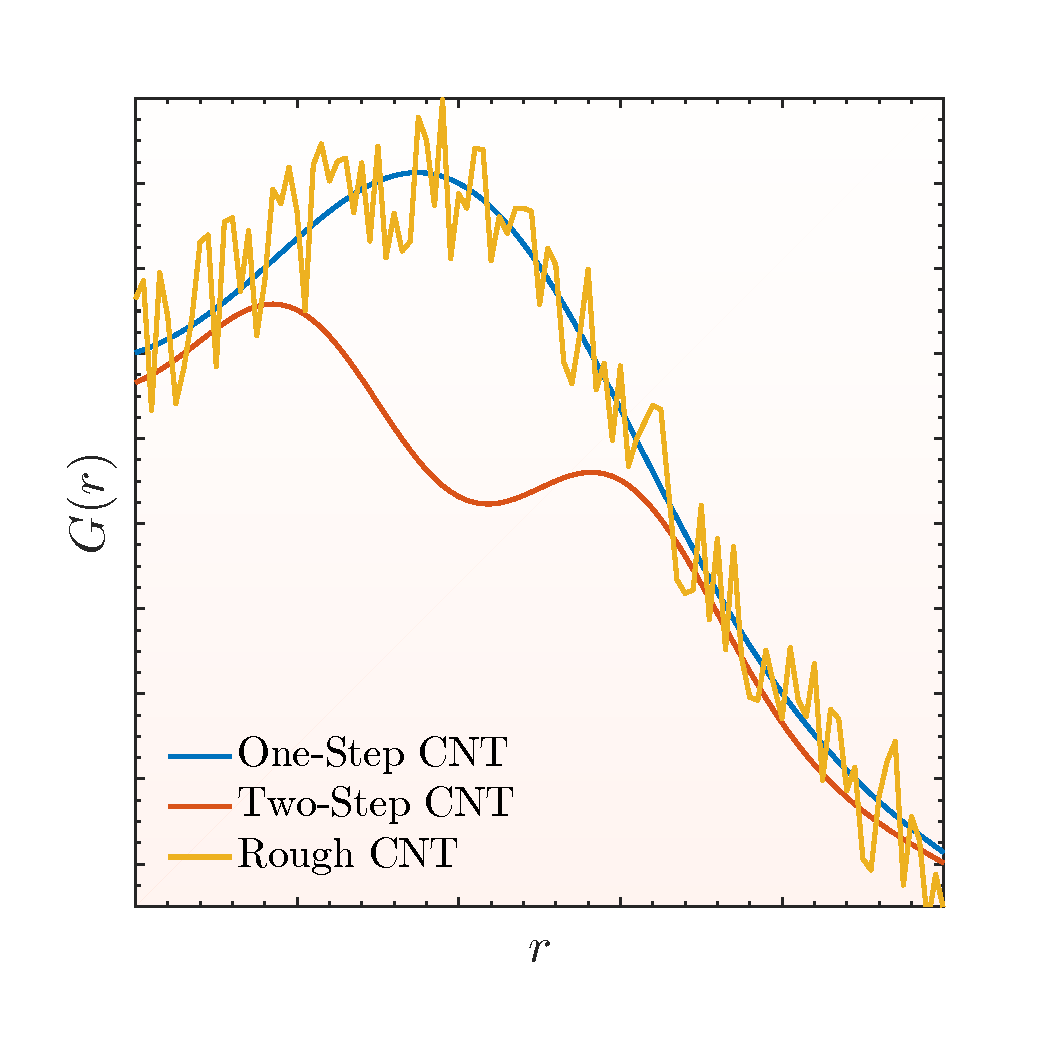
\includegraphics[width = .5\textwidth]{./Figures/CNT/extended_cnt.pdf}
	\caption[Gibbs free energy plotted as a function of reaction coordinate or nucleation site radius.  The blue line is the traditional one-step classical nucleation theory described above.  The red line is the two-step classical nucleation free energy barrier.  In this framework, two free energy barriers separate the bulk phase from the new phase.  The first barrier separates the bulk from a metastable nucleation site, and the second barrier represents internal rearrangements required for the new phase to fully emerge.  The yellow line represents a rough or coarse free energy for nucleation, in which many metastable phases or configurations separate the bulk phase from the stable phase.]{Gibbs free energy plotted as a function of reaction coordinate or nucleation site radius.  The blue line is the traditional one-step classical nucleation theory described above.  The red line is the two-step classical nucleation free energy barrier.  In this framework, two free energy barriers separate the bulk phase from the new phase.  The first barrier separates the bulk from a metastable nucleation site, and the second barrier represents internal rearrangements required for the new phase to fully emerge.  The yellow line represents a rough or coarse free energy for nucleation, in which many metastable phases or configurations separate the bulk phase from the stable phase. \cite{DeYoreo2016}}
	\label{extended_cnt}
\end{figure}

Figure \ref{extended_cnt} shows three different frameworks that extend the theory of classical nucleation theory \cite{DeYoreo2016}.  The simple one-step CNT is the traditional method previously described, in which single monomers cross an interface to either enter the stable phase or enter the metastable phase.  This is believed to be an accurate picture for simple processes such as monoatomic systems condensing, in which single atoms are involved in each step.  A extension of this model is the two step CNT framework, in which two activation barriers separate the two phases with a coexisting metastable phase between the two activation barriers \cite{DeYoreo2016}.  This has been recently seen in many systems.  An example of this, observed in computations, is a supercooled liquid that forms metastable BCC crystallites in the bulk (the first activation barrier).  Then, after the BCC crystallites grow and combine, the solid phase reorders to form an FCC crystal (the second activation barrier) \cite{Braig2011}.  Lastly, the one-step CNT framework was coarsened to create the roughened classical nucleation theory \cite{DeYoreo2016}.  This theory proposes that the general picture of classical nucleation theory is correct, but the overall free energy is rich in small activation barriers and metastable states \cite{DeYoreo2016}.  This picture is applied to substances in which many metastable microscopic states exists in between the initial phase and the final phase, such as the aggregation of polymers or protein folding \cite{DeYoreo2016}\cite{Vekilov2016}.  

Classical nucleation makes very strict assumptions on shape, size, and the uses macroscopic quantities to predict the free energy barrier involved in the nucleation process.  However, as Figure \ref{extended_cnt} shows, the simple approximation that the original classical nucleation theory makes about the free energy barrier is drastically too simple, and as a result, leads to a large errors in nucleation rate predictions.  Ideally, a method to estimate the free energy barrier that is unbiased by assumptions in size, shape, or height of the barrier could be used with classical nucleation theory to make more accurate predictions.  In the following chapters, we will discuss the use of metadynamics simulations to obtain an unbiased estimation of the free energy barrier, and use this barrier to make predictions on the nucleation rate.

